\documentclass[11pt]{article}
\usepackage[a4paper,margin=0.65in]{geometry}
\usepackage[T1]{fontenc}
\usepackage{lmodern}
\usepackage{tikz}
\usetikzlibrary{arrows.meta,positioning,shapes.geometric,fit,calc}
\usepackage{pdflscape}
\usepackage{float}
\usepackage{caption}
\pagestyle{plain}
\setlength{\parindent}{0pt}

\tikzset{
  classbox/.style={draw, rounded corners=2pt, fill=blue!3, align=left,
    font=\small, inner sep=5pt, text width=5.0cm},
  smallclass/.style={draw, rounded corners=2pt, fill=blue!3, align=left,
    font=\small, inner sep=5pt, text width=4.2cm},
  module/.style={draw, rounded corners=3pt, fill=teal!7, align=center,
    minimum height=9mm, text width=3.4cm, font=\small},
  datastore/.style={draw, cylinder, shape border rotate=90, aspect=0.25,
    fill=orange!10, align=center, minimum height=9mm, text width=2.8cm, font=\small},
  decision/.style={diamond, draw, fill=yellow!12, align=center, aspect=2.0,
    inner sep=2pt, font=\small},
  flow/.style={-{Stealth[length=2.2mm]}, thick},
  dependency/.style={-{Stealth[length=2mm]}, dashed, thick},
  association/.style={-{Stealth[length=2mm]}, thick}
}
\begin{document}
\begin{center}
{\LARGE\bfseries Automated Plagiarism Checker}\\[2mm]
{\large Text Processing Flowchart}
\end{center}
\vspace{4mm}

\begin{figure}[H]\centering
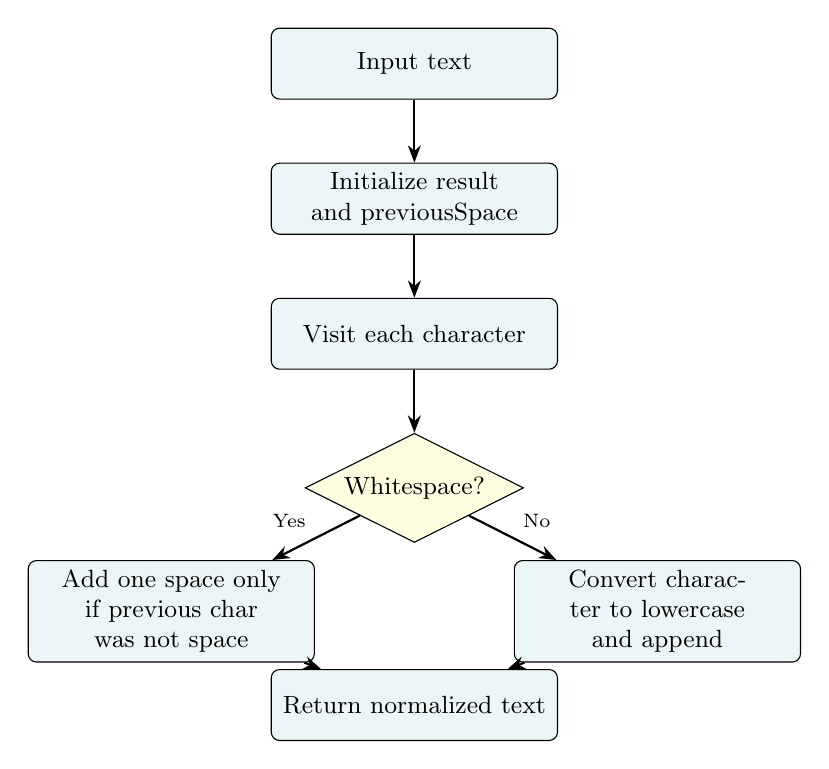
\begin{tikzpicture}[node distance=8mm]
\node[module] (a) {Input text};
\node[module,below=of a] (b) {Initialize result and previousSpace};
\node[module,below=of b] (c) {Visit each character};
\node[decision,below=of c] (d) {Whitespace?};
\node[module,below left=of d] (e) {Add one space only\\if previous char was not space};
\node[module,below right=of d] (f) {Convert character to lowercase\\and append};
\node[module,below=16mm of d] (g) {Return normalized text};
\draw[flow] (a)--(b);
\draw[flow] (b)--(c);
\draw[flow] (c)--(d);
\draw[flow] (d)--node[above left,font=\scriptsize]{Yes}(e);
\draw[flow] (d)--node[above right,font=\scriptsize]{No}(f);
\draw[flow] (e)--(g);
\draw[flow] (f)--(g);
\end{tikzpicture}
\caption{TextProcessor collapses consecutive whitespace and lowercases non-whitespace characters.}
\end{figure}

\end{document}
